\section{Classification Ensembles}
%\begin{figure}[H]
%  \centering
%  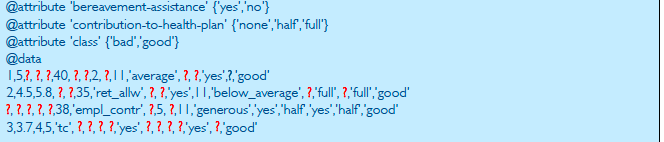
\includegraphics[width=.5\linewidth]{arffmissing}
%\end{figure}

Ensembles generate a \textbf{set of classifiers} from the training data.They predict the class label by \textbf{aggregating} predictions made from \textbf{previous classifiers}
\begin{figure}[H]
  \centering
  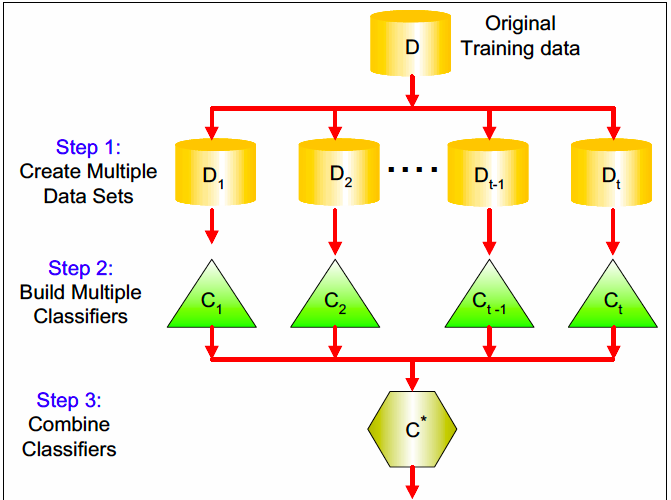
\includegraphics[width=.6\linewidth]{ensemble}
\end{figure}
Using more classifiers and let them vote to decide the outcome often increases performance greatly at the cost of creating hard to analyze structures and outputs.
Assume there are 25 independent classifiers each with error rate $\epsilon= 0.35$
The probability that the ensemble makes an error is :
$$ \sum \limits_{i=1}^{25} \binom{25}{i}\epsilon^i(1-\epsilon)^{25-i}= 0.06$$
How can classifiers be independent is they train on the same dataset?

\subsection{Bagging}
Given a set D of d tuples, at each iteration i ,a training set $D_i$ of tuples is sampled with replacement from D (\textbf{bootstrap}).Then a \textbf{classifier} $M_i$ is learned for each training set $D_i$.\\
Prediction is performed by taking all outputs of the classifier and assigns the class with the \textbf{most votes}. This gives equal weight to each classifier.\\
This approach can also be applied to \textbf{regression} by taking the \textbf{average of the votes}.\\
Bagging works because it \textbf{reduces the variance} by voting/averaging but  \textbf{cannot always be applied}:
\begin{itemize}
\item if the learning algorithm is \textbf{unstable} (small changes in training set cause big changes in classifier) ,bagging almost always increases performance. 
Good for NN ,DT, Regression Trees, Linear Regression...
\item if the learning algorithm is stable (example : KNN ) using bagging is a bad idea.
\end{itemize}

\subsection{Algorithm Randomization}
Instead of randomizing data , the algorithm itself can sometimes be randomized: 
\begin{itemize}
\item weights in NN can be randomized
\item attribute selection or confidence level for pruning in DT can be randomized. The more \textbf{uncorrelated the trees} the greater the \textbf{variance reduction}.
\item ...
\end{itemize}
Often randomizing the algorithm can be used in combination with \textbf{bagging}. 

\subsubsection{Random Forests}
It is a learning ensemble consisting of a \textbf{bagging}  of unpruned \textbf{decision tree learners} with \textbf{randomized selection of features} at each split. The \textbf{generalization error} of a RF depends on the \textbf{individual strength} of the trees and the \textbf{correlation} between them.
\begin{figure}[H]
  \centering
  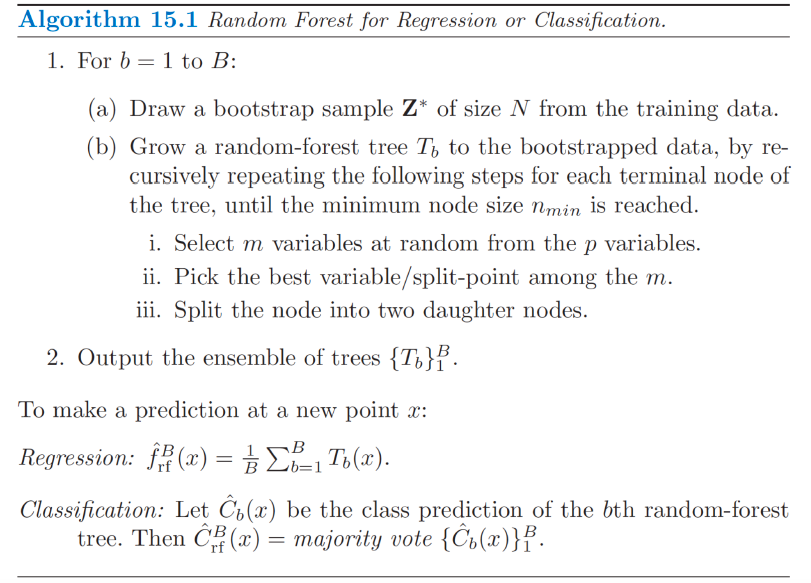
\includegraphics[width=.7\linewidth]{RF}
\end{figure}
Random forest have an amazing feature called \textbf{Out-of-bag Evaluation} , a method to evaluate performance without using \textbf{cross-validation} :
for each observation $(x_i,y_i)$ construct its random forest predictor by \textbf{averaging} only those trees corresponding to bootstrap samples in which the observation \textbf{did not appear}. This can be done during the \textbf{fitting phase}!\\
RF are very easy too use, as they require only few parameters to set up , but have a \textbf{high accuracy} and are good ad avoiding \textbf{overfitting} by choosing a high number of trees. Additional properties:
\begin{itemize}
\item Returns variable importance estimates
\item A excellent in classification , not so excellent in regression
\item Gains accuracy if used with boosting 
\end{itemize}

\subsection{Boosting}
Boosting consists in making a final prediction working on the errors of previous learners. The first boosting method used is \textbf{AdaBoosting}.
\begin{enumerate}
\item Assign weights to each training example
\item Learn iteratively k classifiers
\item After classifier $M_i$ is learned the weights are updated to allow the subsequent classifier $M_{i+1}t$ to pay more attention to the training tuples that were missclassified by $M_i$.
\item The final $M_*$ combines the votes of each individual classifier where the weight of each classifier's vote is a function of its accuracy.
\end{enumerate}
Boosting work with \textbf{weak classifiers} , as long as the error \textbf{does not exceed 0.5}. Also boosting \textbf{can lead to overfitting}.

\subsubsection{AdaBoosting}
AdaBoost computes a \textbf{strong classifier} as a combination of a week classifier 
$$ H(x) = sign \left(  \sum \limits_{t=1}^{T} \alpha_t h_t(x) \right)$$
where 
\begin{itemize}
\item $h_t(x) $ is the output of weak classifier t
\item $\alpha_t$ is the weight assigned to classifier t from its \textbf{estimated error } $\epsilon_t$:
$$ \alpha_t = \frac{1}{2} ln \left( \frac{1-\epsilon_t}{\epsilon_t} \right)$$
\end{itemize}

The weights are update by multiplying them by :
\begin{itemize}
\item $e^{-\alpha}$ if correctly classified
\item $e^{\alpha}$ if incorrectly classified
\end{itemize}
While the error rate is computed as :
$$ \epsilon_i = \frac{1}{N} \sum \limits_{j=1}^{N}w_j \delta(h_i(x_j) \neq y_i)$$
\begin{figure}[H]
  \centering
  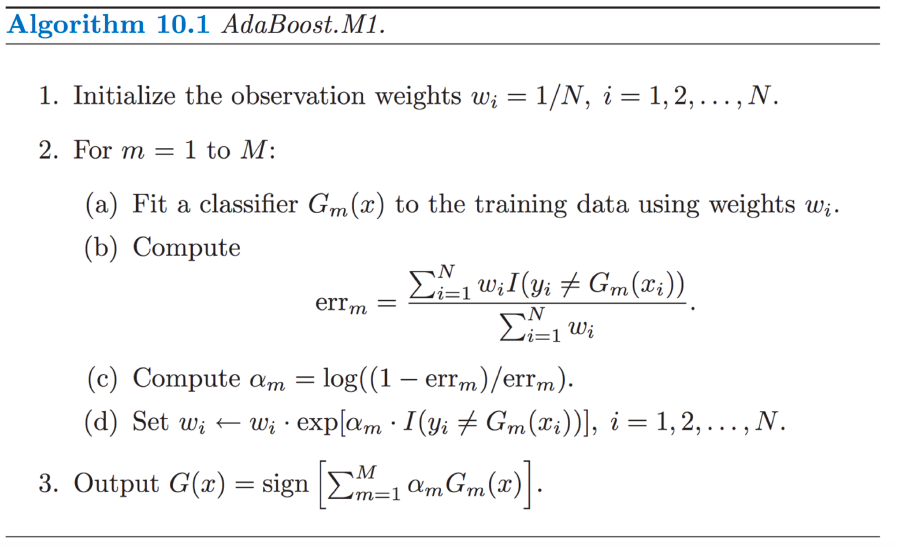
\includegraphics[width=.6\linewidth]{adaboost}
\end{figure}
Example of adaboost
\begin{figure}[H]
  \centering
  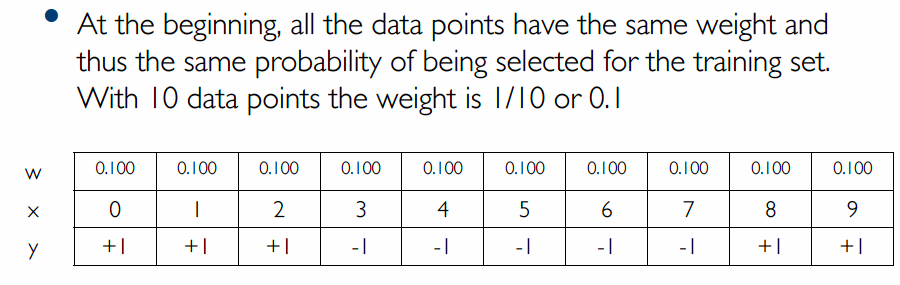
\includegraphics[width=.6\linewidth]{ada1}
\end{figure}
\begin{figure}[H]
  \centering
  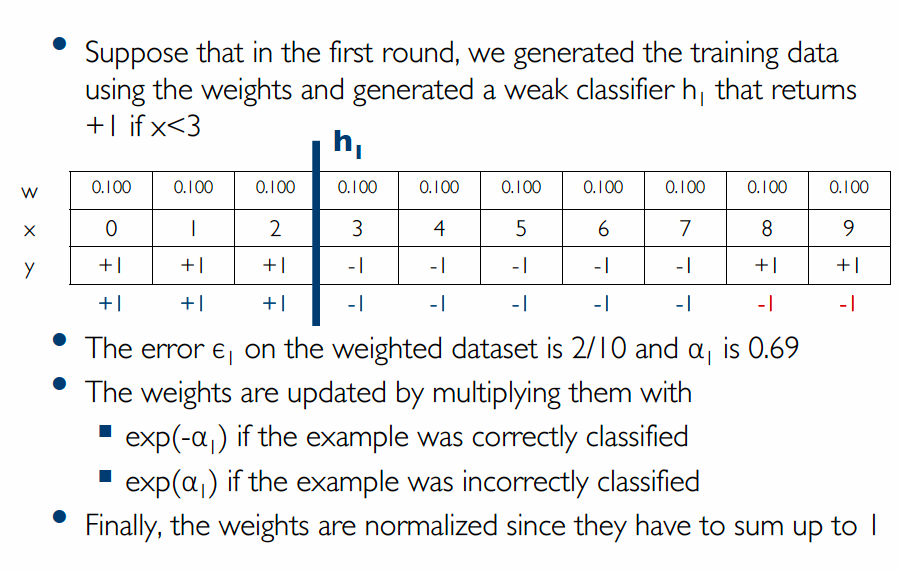
\includegraphics[width=.6\linewidth]{ada2}
\end{figure}
\begin{figure}[H]
  \centering
  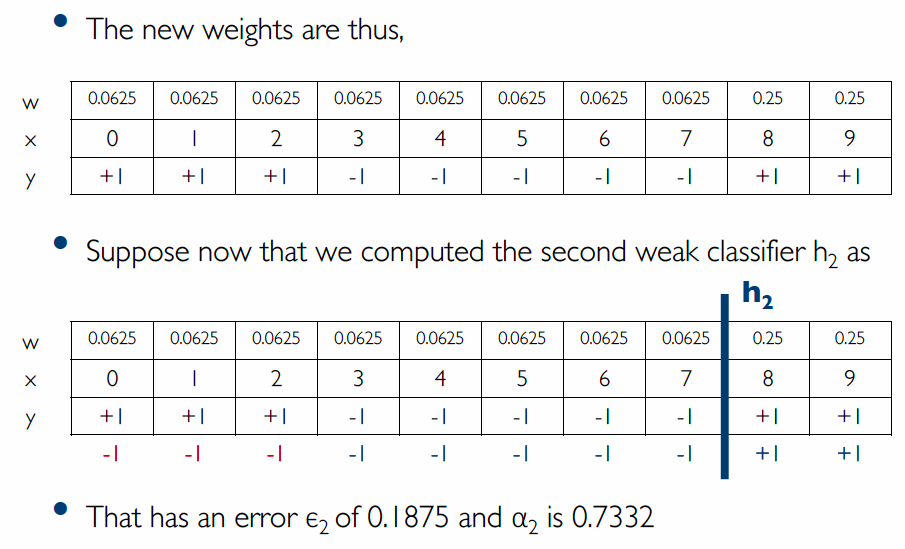
\includegraphics[width=.6\linewidth]{ada3}
\end{figure}
And so on.\\

\subsubsection{Boosting Stumps}
Boosting can also be used in a Random Forest contest. A weak learner in this contest is the \textbf{decision stump} ,a simple one node DT. A good thing in boosting is that it continues to reduce the \textbf{test error} even if the training error is \textbf{already 0} :this suggests that boosting does not use the training error as basis for learning its trees.

\subsubsection{Gradient Boosting}
Easier to understand for regression but largely used in classification. In summary:
\begin{enumerate}
\item Learn a regression predictor
\item Compute the error residual
\item \textbf{Learn to predict the residual}
\item Repeat 2-4 
\end{enumerate}
The sum of predictions is increasingly accurate while the predictive function get more and more complex.
Example on the MSE:
\begin{itemize}
\item To compute a model to predict target value $y_i$ that minimizes a loss function like MSE $$ MSE(y,\hat{y}) = \frac{1}{N}\sum \limits_{i=1}^{N}(y_i - \hat{y_i})^2$$
\item Adjust $\hat{y_i}$ to try to reduce the error using gradient 
$$ \hat{y_i} = \hat{y_i} + \alpha \nabla MSE(y,\hat{y})$$
Where the gradient is a function of $y_i - \hat{y_i}$
\end{itemize}
Each learner tries to estimate the gradient for the loss.
\begin{figure}[H]
  \centering
  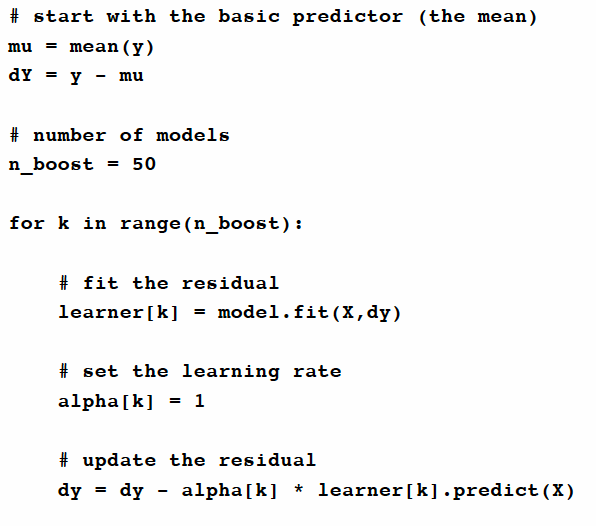
\includegraphics[width=.6\linewidth]{gb1}
\end{figure}\begin{figure}[H]
  \centering
  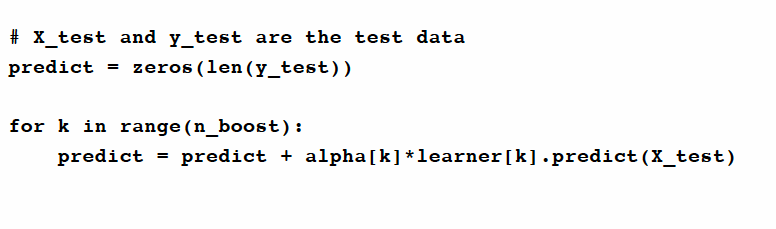
\includegraphics[width=.6\linewidth]{gb2}
\end{figure}

\subsubsection{eXtreme Gradient Boosting}
Efficient  and scalable implementation of gradient boosting applied to classification and regression trees. \textbf{Only deals with numerical variables} (use \textbf{CatBoosting} for categorical data).\\
Its main advantages are that it is very fast wrt to normal gradient boosting as it uses:
\begin{itemize}
\item novel tree learning algorithm to handle \textbf{sparse data}
\item approximate learning using \textbf{quantile sketch}
\item more regularized model formalization to control \textbf{overfitting}
\end{itemize}

\subsection{Learning Ensembles}
Learning ensembles steal the idea behind RF and Boosting by building \textbf{stonger models} by performing a global optimization over the ensemble.
\begin{itemize}
\item Generate a \textbf{dictionary of models} :
$$ D = \{ T_1(X) ,T_2(X) ,...,T_M(X) \}$$
\item Fit a model to the data
$$ F(X) = \sum \limits_{\alpha \in D} \alpha_mT_m(X)$$
\end{itemize}
Stacking generalization  train a learning algorithm to combine predictions of \textbf{heterogeneous} set of learning algorithms:
\begin{itemize}
\item Train a set of base learners over the data 
\item Use a \textbf{meta learner} that is trained using the predictions of the base classifiers as additional inputs
\end{itemize}
Apply CV